\documentclass[11pt,a4paper]{article} 

\usepackage[utf8]{inputenc}
\usepackage[T1]{fontenc}
\usepackage[margin=1.5cm]{geometry}
\usepackage{lmodern}
\usepackage{microtype}
\usepackage{hyperref}
\usepackage{booktabs}
\usepackage{listings}
\usepackage{xcolor}
\usepackage{parskip}
\usepackage{titlesec}
\usepackage{enumitem}
\usepackage{amssymb}
\usepackage{setspace}
\usepackage{amsmath}
\usepackage{tikz}
\usepackage{pgfplots}
\pgfplotsset{compat=1.18}

\setlength{\parskip}{3pt} 
\setlength{\parindent}{0pt}
\singlespacing

\DeclareUnicodeCharacter{2752}{$\blacksquare$} 
\DeclareUnicodeCharacter{2751}{$\square$} 

\lstdefinelanguage{Python}{
  keywords={import, from, class, def, return, if, else, elif, while, for,
            in, and, or, not, True, False, None, try, except, raise, yield,
            lambda, with, as, pass, break, continue, property},
  keywordstyle=\color{blue}\bfseries,
  comment=[l]{\#},
  commentstyle=\color{gray}\itshape,
  stringstyle=\color{teal},
  basicstyle=\ttfamily\footnotesize,
  breaklines=true,
  frame=single,
  rulecolor=\color{black!25},
  backgroundcolor=\color{black!4},
  tabsize=4,
  showstringspaces=false
}
\lstset{language=Python}

\titleformat{\section}{\bfseries}{}{0em}{}[\titlerule]
\titleformat{\subsection}{\normalsize\bfseries}{}{0em}{}
\titlespacing*{\section}{0pt}{8pt}{4pt}
\titlespacing*{\subsection}{0pt}{6pt}{3pt}

\setlist{nosep, leftmargin=*}
\renewcommand{\arraystretch}{0.9}

\begin{document}

\begin{titlepage}
    \centering
    \vspace*{2cm}
    
    {\LARGE \textbf{Introdução à Inteligência Artificial}}\\[8pt]
    {\Large Data Science Degree}\\[4pt]
    {\large NOVA IMS}\\[1.5cm]
    
    {\Huge \textbf{Artificial Life Simulation Engine}}\\[0.8cm]
    {\Large \textbf{Evolutionary Dynamics of Zizoids (Prey) and Wsiloids (Predators)}}\\[2.0cm]
    
    \rule{0.8\textwidth}{0.4pt}\\[0.5cm]
    {\Large \textbf{Author}}\\[6pt]
    {\Large Malvin Tafadzwa Chitswamatombo (20250870)}\\[2cm]
    
    {\large June 2026}
    
    \vfill
\end{titlepage}

\newpage

\section{Introduction}

The goal of this project is to model and simulate an artificial life (ALife) environment consisting of two virtual beings in a 2D spatial world: **Zizoids** (Prey) who must survive, consume food, and reproduce, and their predators, **Wsiloids** (Predators), who hunt them. The Zizoids are equipped with a feed-forward Artificial Neural Network (ANN) as a brain, directly connecting their vision and stomach (hunger) inputs to motor output commands. Over generations, Zizoids undergo natural selection where fit individuals pass on their genetic parameters, leading to adaptive behaviors such as escaping predators and foraging food.

\subsection{Codebase Structure}
The codebase is divided into several modules inside the \texttt{Alife\_Simulation/} project folder:
\begin{itemize}
    \item \texttt{game.py} - The Director and main execution script. It manages high-level logic loops, user interactions, serialization, and logging.
    \item \texttt{code/graphics.py} - The dashboard visualization manager. Handles Pygame display initialization, rendering the 2D grid, drawing graphs, and showing performance statistics.
    \item \texttt{code/world.py} - The spatial stage manager that handles spatial sync, movement bounds, collision resolution, reproduction handshakes, and resource growth.
    \item \texttt{code/prey.py} - The representation of Prey (Zizoids). Includes age-dependent Gaussian capacities, logarithmic growths, survival rolls, vision vectors, and motor mappings.
    \item \texttt{code/ANNprey.py} - Pure mathematical implementation of the feed-forward neural network brain.
    \item \texttt{code/predator.py} - Heuristic state machine for Wsiloids, featuring a proximity chase reflex and erratic random search.
    \item \texttt{code/food.py} - Passive cacao resources that sprout and compound in nutritional value over time.
\end{itemize}

\subsection{How to Run}
Execute the following in the terminal:
\begin{lstlisting}[language=bash]
python Alife_Simulation/game.py
\end{lstlisting}
The program opens with a console boot menu allowing you to: (1) load a previous checkpoint (\texttt{simulation\_state.json}), (2) run the default configuration (using default starting counts and grid sizes), or (3) configure custom parameters. Once booted, it launches a Pygame visual dashboard. The user can pause the simulation using \texttt{[SPACE]}, accelerate or decelerate frames using \texttt{[UP Arrow]} and \texttt{[DOWN Arrow]}, save checkpoints on demand using \texttt{[S]}, or quit using \texttt{[ESC]}.

\section{Real-Time UI \& Dashboard}

The visual dashboard in \texttt{code/graphics.py} renders a dual-panel screen with a charcoal-black background:
\begin{itemize}
    \item \textbf{Left Panel (Environment Grid):} Renders the grid matrix where cells represent spatial states. Crimson Red ellipses denote Wsiloids (Predators), Forest Green rects denote Food (cacao), and Electric Blue ellipses denote Zizoids (Prey). Inside each Zizoid circle, a white heading line points in the direction of its current orientation (North, East, South, West).
    \item \textbf{Right Panel (Dashboard Monitor):} Displays real-time state metrics, including the current Tick count, FPS, and entity counts. It includes a **Fitness Breakdown** showing the minimum, median, and maximum (elite) scores of the prey population based on age. It also shows a **Global Traits Monitor** indicating moving averages of energy, intelligence, and efficiency, followed by a **Population Graph** plotting Prey (blue), Predator (red), and Food (green) historical sizes over a rolling window.
\end{itemize}
The simulation saves its state in JSON format to \texttt{simulation\_state.json} and logs statistics to \texttt{simulation\_1.csv} in append mode at regular logging intervals. The logs record variables like population counts, average energy, average intelligence, average efficiency, and the serialized chromosome of the elite individual. If the Zizoid population reaches zero, the simulation halts and prints a final audit.

\section{Prey (Zizoid) Modeling \& The Neural Brain}

Each Zizoid is governed by a deterministic, feed-forward Artificial Neural Network (ANN) defined in \texttt{ANNprey.py}. The design of this network draws from principles in the \textit{Ghana Forest} midge behavior model codebase \cite{ghanaforest}, where perception inputs map to actions via a sigmoid hidden layer. For the more complex neural and genetic network applications, Lenny Malard's \textit{NEAT from Scratch} implementation \cite{neatfromscratch} served as a major reference.

\subsection{Vision and Hunger Sensory Inputs}
The Zizoid perceives its surroundings through concentric vision rings oriented relative to its current heading. As its intelligence grows, its sensory reach extends farther out, expanding its active vision radius. Instead of dynamically restructuring the neural brain network when the agent's vision radius changes (which would corrupt inherited connections), the network maintains a fixed sensory dimension (see Appendix~\ref{sec:ann_params} for exact inputs). Rings that are beyond the agent's current intelligence-restricted sight limit are masked (zero-padded) in the input layer.

In addition to spatial vision, the Zizoid receives an internal metabolic signal representing hunger. This hunger sensor is a continuous scalar value reflecting the agent's current energy reserve relative to its base energy capacity, allowing it to adapt its behavior when starving.

\subsection{Brain Computations and Chromosome Mapping}
The neural network brain processes the sensory inputs through hidden layer units, mapping them to action probabilities. Over generations, the weights and biases of this neural network are encoded as a flat list of genes, constituting the Zizoid's chromosome. In addition to neural network weights, the chromosome codes for base traits such as efficiency and intelligence. Fitter individuals pass on their chromosomes, and mutations introduce small random variations, driving the evolution of complex adaptive behaviors.

\subsection{Locomotion and Action Selection}
The motor command outputs control relative muscle translations, driving the agent to move in directions relative to its current heading (such as diagonal strides, forward steps, backward adjustments, rotation, or remaining stationary). These relative steps are resolved into absolute grid displacements depending on the agent's orientation. To model biological momentum and fatigue, diagonal moves utilize an alternating jump check cadence, allowing Zizoids to run at a higher average velocity. The relative locomotion command options are illustrated in Figure~\ref{fig:locomotion}.

\begin{figure}[ht]
\centering
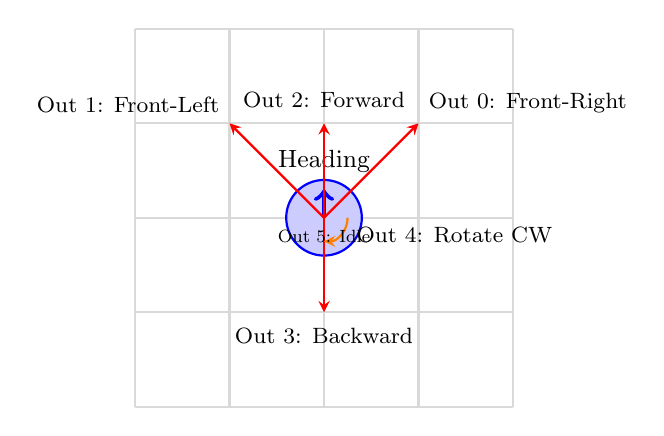
\begin{tikzpicture}[scale=1.2]
    \draw[thick, step=1cm, gray!30] (-2,-2) grid (2,2);
    % Draw midge at center
    \draw[fill=blue!20, draw=blue, thick] (0,0) circle (0.4cm);
    \draw[->, ultra thick, blue] (0,0) -- (0,0.3) node[above=2pt, black] {\small Heading};
    % Draw relative offsets
    \draw[->, thick, red, >=stealth] (0,0) -- (1,1) node[above right, black] {\footnotesize Out 0: Front-Right};
    \draw[->, thick, red, >=stealth] (0,0) -- (-1,1) node[above left, black] {\footnotesize Out 1: Front-Left};
    \draw[->, thick, red, >=stealth] (0,0) -- (0,1) node[above=2pt, black] {\footnotesize Out 2: Forward};
    \draw[->, thick, red, >=stealth] (0,0) -- (0,-1) node[below=2pt, black] {\footnotesize Out 3: Backward};
    \draw[->, thick, orange, >=stealth] (0.25,0) arc (0:-90:0.25cm) node[right=2pt, midway, black] {\footnotesize Out 4: Rotate CW};
    \node at (0, -0.2) [scale=0.8, black] {\footnotesize Out 5: Idle};
\end{tikzpicture}
\caption{Relative Locomotion Map for Zizoid Muscle Activations.}
\label{fig:locomotion}
\end{figure}

\section{Genetics, Lifespan Dynamics \& Selection}

\subsection{Expected Lifespan and Gaussian Scaling}
The baseline expected lifespan ($LE$) of Zizoids is determined dynamically by global simulation parameters, including the initial energy and the population counts of prey and predators. The Zizoid's maximum energy capacity and its reproduction probability are scaled dynamically using a Gaussian curve that peaks at mid-life. To protect young or old individuals from dying immediately upon spawning, a protective minimum floor is applied to the energy capacity multiplier.

\subsection{Logarithmic Growth of Base Traits}
Base traits (efficiency and intelligence) scale logarithmically with age, modeling experience accumulation. Reaching specific intelligence milestones scales the active vision radius of the Zizoid, expanding its sensory reach.

\subsection{Logarithmic Decay of Survival Probability}
The probability of surviving a single step decays logarithmically as the agent ages. The decay rate is calculated such that the cumulative probability of surviving to the expected lifespan is exactly half, representing natural aging and preventing immortal agents. The curves representing lifecycle factors, trait growth, and survival decay are visualized in Figure~\ref{fig:curves} and Figure~\ref{fig:survival}.

\begin{figure}[h]
\centering
\begin{minipage}{0.48\textwidth}
\centering
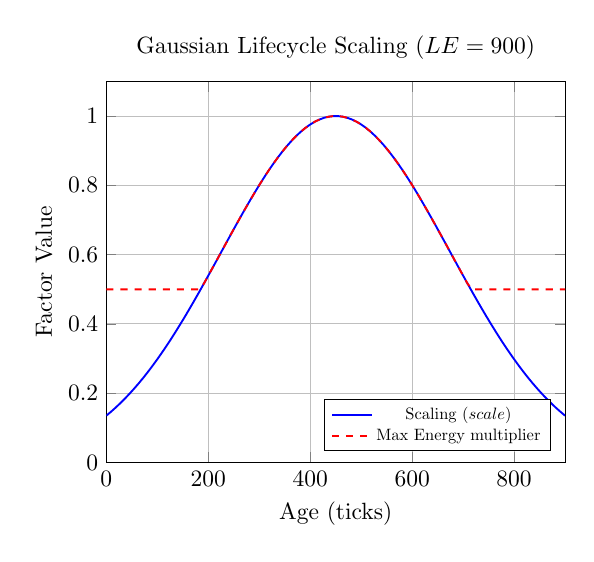
\begin{tikzpicture}[scale=0.85]
\begin{axis}[
    title={Gaussian Lifecycle Scaling ($LE = 900$)},
    xlabel={Age (ticks)},
    ylabel={Factor Value},
    xmin=0, xmax=900,
    ymin=0, ymax=1.1,
    grid=both,
    legend pos=south east,
    legend style={nodes={scale=0.7, transform shape}}
]
\addplot[blue, thick, domain=0:900, samples=100] {exp(-0.5*((x - 450)/225)^2)};
\addlegendentry{Scaling ($scale$)}
\addplot[red, dashed, thick, domain=0:900, samples=100] {max(0.5, exp(-0.5*((x - 450)/225)^2))};
\addlegendentry{Max Energy multiplier}
\end{axis}
\end{tikzpicture}
\end{minipage}
\hfill
\begin{minipage}{0.48\textwidth}
\centering
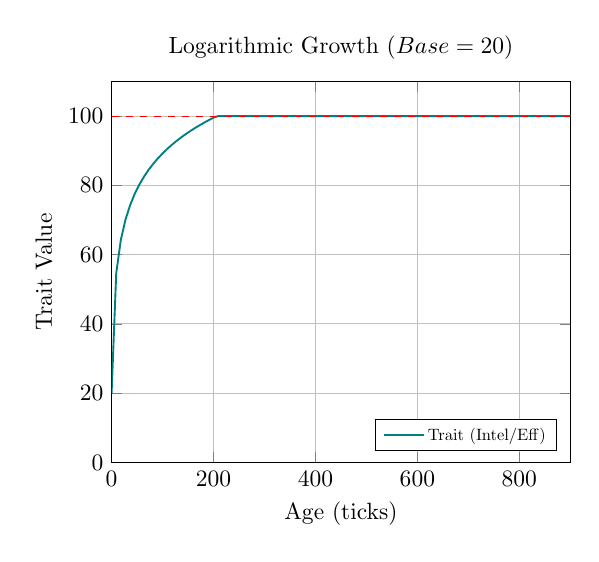
\begin{tikzpicture}[scale=0.85]
\begin{axis}[
    title={Logarithmic Growth ($Base = 20$)},
    xlabel={Age (ticks)},
    ylabel={Trait Value},
    xmin=0, xmax=900,
    ymin=0, ymax=110,
    grid=both,
    legend pos=south east,
    legend style={nodes={scale=0.7, transform shape}}
]
\addplot[teal, thick, domain=0:900, samples=100] {min(100, 20 + 15*ln(x+1))};
\addlegendentry{Trait (Intel/Eff)}
\draw[dashed, red] (axis cs:0,100) -- (axis cs:900,100);
\end{axis}
\end{tikzpicture}
\end{minipage}
\caption{Visualization of Lifespan Metrics and Logarithmic Growth curves.}
\label{fig:curves}
\end{figure}

\begin{figure}[h]
\centering
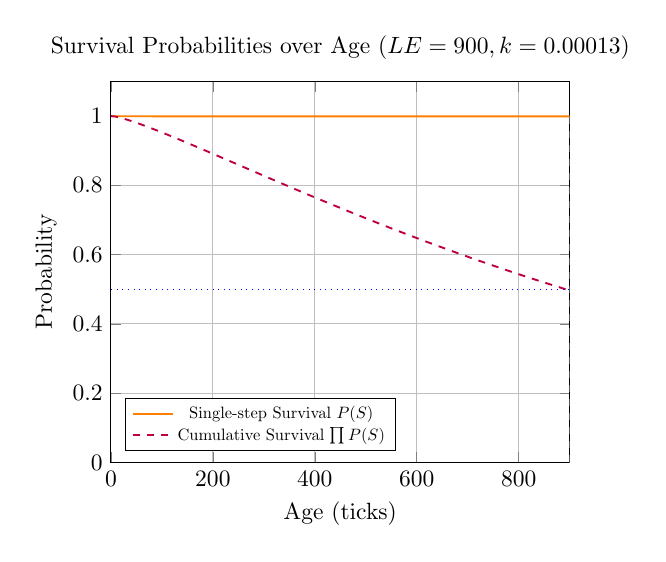
\begin{tikzpicture}[scale=0.85]
\begin{axis}[
    title={Survival Probabilities over Age ($LE=900, k=0.00013$)},
    xlabel={Age (ticks)},
    ylabel={Probability},
    xmin=0, xmax=900,
    ymin=0, ymax=1.1,
    grid=both,
    legend pos=south west,
    legend style={nodes={scale=0.7, transform shape}}
]
\addplot[orange, thick, domain=0:900, samples=100] {max(0.0, 1.0 - 0.000134 * ln(x+1))};
\addlegendentry{Single-step Survival $P(S)$}
\addplot[purple, dashed, thick, domain=0:900, samples=100] {exp(-0.000134 * (x*ln(x+1) - x))};
\addlegendentry{Cumulative Survival $\prod P(S)$}
\draw[dashed, gray] (axis cs:900,0) -- (axis cs:900,1.0);
\draw[dotted, blue] (axis cs:0,0.5) -- (axis cs:900,0.5);
\end{axis}
\end{tikzpicture}
\caption{Single-step and cumulative survival decay. The cumulative survival decays to $\approx 50\%$ at $LE$.}
\label{fig:survival}
\end{figure}

\subsection{Selection, Reproduction, and Crossover}
Natural selection is implemented via **Darwinian Local Mate Selection**. When two Zizoids are adjacent, they perform a mating handshake. If they mate, both enter a gestation period where they remain stationary and consume energy. To choose the second parent's genetic contributions, the system searches the grid within a local neighborhood to select the individual with the highest fitness based on age, food consumption, and reproduction history. The child's chromosome is formed via crossover and mutation. The crossover strategies alternate functional blocks or split genes at random pivots, and Gaussian mutation introduces small adjustments to neural weights.

\section{Predator (Wsiloid) Heuristics \& Spatial Dynamics}

Predators (Wsiloids) are governed by a heuristic state machine implemented in \texttt{predator.py}. They have no genetic code and do not age-decay.

\subsection{Locomotion and Targeting Heuristic}
Wsiloids target prey via a proximity chase exception. They check their immediate neighborhood: if a Zizoid is present, they enter a chase state and run directly toward the target. If no Zizoid is adjacent, they step erratically into empty or resource-containing tiles.

\subsection{Combat Catch Tax and Escape Mechanics}
When a Wsiloid steps on a cell occupied by a Zizoid, a collision catch resolution is triggered:
\begin{itemize}
    \item \textbf{Combat Tax:} The Zizoid is immediately hit with a heavy energy cost.
    \item \textbf{Catch Case:} If the Zizoid's energy falls below zero, it dies and is removed. The Wsiloid gains energy, and its tracking efficiency is boosted.
    \item \textbf{Escape Case:} If the Zizoid survives, it escapes. To model the evolutionary advantage of surviving a predator attack, the Zizoid receives a permanent experience boost to its base attributes in its chromosome. Conversely, the Wsiloid suffers an efficiency penalty, loses energy, and the Zizoid is pushed to the nearest empty cell.
\end{itemize}
Additionally, Wsiloids crush and exhaust food cells when stepping on them. An environmental stabilizer respawns predators if their population drops below initial defaults.

\section{Design Evolution: Brainstorming vs. Final Implementation}

The final codebase reflects a series of design adjustments made to adapt the initial unstructured brainstorming into a stable, running biological simulation. This section details the comparison between the initial concepts and their final implementation, providing the engineering rationales behind these transitions.

\subsection{Spatial Density Constraints and Sudoku Spacing}
\begin{itemize}
    \item \textbf{Brainstorming concept:} Spawning predators such that no two predators occupy the same row or column initially (Sudoku constraint), with a safety buffer between predator and prey.
    \item \textbf{Final implementation:} Spawning Wsiloids using modular stride coordinates. If the predator count exceeds the grid width or height, the pigeonhole principle prevents absolute row/column uniqueness.
    \item \textbf{Justification:} The modular stride algorithm distributes predators evenly across the grid to approximate unique spacing. Safety buffers and floor-fill food placement are fully preserved. The spacing grid layout is illustrated in Figure~\ref{fig:sudoku}.
\end{itemize}

\begin{figure}[ht]
\centering
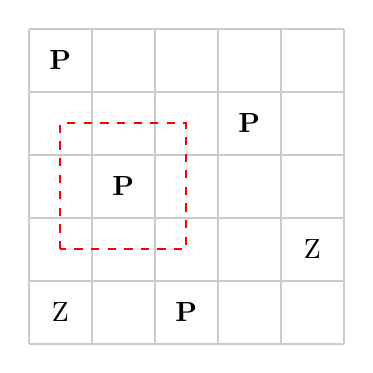
\begin{tikzpicture}[scale=0.8]
    \draw[thick, step=1cm, gray!40] (0,0) grid (5,5);
    % Spacing out predators (P) modularly:
    \node at (0.5, 4.5) {\textbf{P}}; 
    \node at (3.5, 3.5) {\textbf{P}}; 
    \node at (1.5, 2.5) {\textbf{P}}; 
    \node at (2.5, 0.5) {\textbf{P}}; 
    % Prey (Z) with 1-cell buffer shown
    \node at (0.5, 0.5) {Z};
    \node at (4.5, 1.5) {Z};
    % Draw buffer zone around one predator at (1.5, 2.5)
    \draw[red, dashed, thick] (0.5,1.5) rectangle (2.5,3.5);
\end{tikzpicture}
\caption{Modular Stride Spacing Grid. Predators (P) are distributed deterministically across rows and columns to approximate Sudoku uniqueness. The dashed line denotes the 1-cell safety buffer for Prey (Z) spawns.}
\label{fig:sudoku}
\end{figure}

\subsection{Resource Growth and Compounding Buffs}
\begin{itemize}
    \item \textbf{Brainstorming concept:} Food sprouts quickly, compounding nutritional value per step.
    \item \textbf{Final implementation:} Food sprouts after a set unstepped interval and compounds linearly.
    \item \textbf{Justification:} A very low sprout interval flooded the environment with food, removing starvation pressures. Increasing the sprout cooldown successfully restored food scarcity and natural selection.
\end{itemize}

\subsection{Pure Neural Autonomy vs. Pathfinding Overrides}
\begin{itemize}
    \item \textbf{Brainstorming concept:} Prey should combine global pathfinding (like $A^*$) with local neural networks.
    \item \textbf{Final implementation:} Prey movement is governed entirely by the feed-forward neural brain.
    \item \textbf{Justification:} Overriding the brain with hardcoded target pathfinding removes evolutionary pressure. Retaining the neural network as the sole decision-maker forces the genetic algorithm to discover survival behaviors organically.
\end{itemize}

\subsection{Chase Reflex and Evolutionary Arms Race}
\begin{itemize}
    \item \textbf{Brainstorming concept:} Escape boosts prey traits, catches boost predator efficiency.
    \item \textbf{Final implementation:} Escape awards a permanent boost to prey attributes, while catches reward predators.
    \item \textbf{Justification:} This co-evolutionary loop prevents static behaviors, modeling an active co-evolutionary arms race.
\end{itemize}

\subsection{Metabolic Energy Cost Calibrations}
\begin{itemize}
    \item \textbf{Brainstorming concept:} Generational decay drains energy, moving and running consume energy, reproduction has a movement energy cost.
    \item \textbf{Final implementation:} Metabolic decay parameters are scaled.
    \item \textbf{Justification:} Initial low metabolic costs allowed zizoids to walk randomly and survive indefinitely. Scaling costs forces the neural network to develop highly active, efficient foraging strategies.
\end{itemize}

\section{Data Analysis and Simulation Trends}

The simulation dynamics recorded in the CSV logs demonstrate three distinct phases:
\begin{enumerate}
    \item \textbf{Phase 1: Initial Boom and Competition:} Due to abundant food at startup (which floor-fills all non-agent cells), the Zizoid population expands rapidly. High density triggers reproduction.
    \item \textbf{Phase 2: Predator-Prey Oscillation:} As prey count peaks, predators easily trigger adjacent catch states. Predator energy increases, leading to hunting pressure. Prey count decreases, which triggers food regrowth.
    \item \textbf{Phase 3: Trait Adaptation and Stabilization:} The average intelligence and efficiency of Zizoids rise logarithmically. Zizoids evolve to recognize food and run away from predators, increasing their average lifespan. The system settles into a dynamic equilibrium until resource exhaustion triggers extinction.
\end{enumerate}

\section{Conclusion}

This artificial life simulation engine integrates neural network brains, genetic algorithms, and spatial heuristics into a cohesive ecosystem. The engineering design decisions—such as the static input neural network mapping to handle dynamic vision masking, the Gaussian-scaled capacities, local Darwinian selection, and the combat tax escape feedback loop—create a stable simulation that models biological natural selection.

\newpage

\appendix

\section{Appendix A: Mathematical Formulations}

\subsection{Neural Brain Computations}
The feed-forward neural brain processes inputs through hidden layer units, mapping them to outputs using the following calculations:
\begin{align}
    \mathbf{h} &= \sigma(\mathbf{W}_h \mathbf{x} + \mathbf{b}_h) \\
    \mathbf{y} &= \text{softmax}(\mathbf{W}_o \mathbf{h} + \mathbf{b}_o)
\end{align}
where $\mathbf{x} \in \mathbb{R}^{81}$ is the input vector, $\mathbf{h} \in \mathbb{R}^8$ is the hidden layer activation vector, $\mathbf{y} \in \mathbb{R}^6$ represents the probability distribution over the 6 actions, $\mathbf{W}_h$ and $\mathbf{W}_o$ are weight matrices, $\mathbf{b}_h$ and $\mathbf{b}_o$ are biases, and $\sigma(z) = 1.0 / (1.0 + e^{-z})$ is the Sigmoid activation function.

To translate relative commands $(r_x, r_y)$ to absolute grid offsets $(dx, dy)$, the system uses the heading angle $\theta \in \{0, 1, 2, 3\}$ representing North, East, South, and West:
\begin{equation}
    (dx, dy) = \begin{cases}
        (r_x, -r_y), & \text{if } \theta = 0\text{ (North)} \\
        (r_y, r_x), & \text{if } \theta = 1\text{ (East)} \\
        (-r_x, r_y), & \text{if } \theta = 2\text{ (South)} \\
        (-r_y, -r_x), & \text{if } \theta = 3\text{ (West)}
    \end{cases}
\end{equation}

\subsection{Expected Lifespan and Lifecycle Scaling}
The baseline expected lifespan ($LE$) of Zizoids is calculated as:
\begin{equation}
    LE = \text{INITIAL\_ENERGY\_PREY} \times \left(1.0 + \frac{N_{\text{prey}}}{N_{\text{predator}} + 1.0}\right)
\end{equation}
The Zizoid’s max energy capacity and reproduction probability scale dynamically:
\begin{align}
    scale(Age) &= \exp\left( -0.5 \left( \frac{Age - LE/2}{LE/4} \right)^2 \right) \\
    E_{\text{max}}(Age) &= E_{\text{init}} \times \max(0.50, scale(Age)) \\
    P_{\text{reproduction}}(Age) &= P_{\text{base\_rep}} \times scale(Age)
\end{align}

\subsection{Experience Growth and Vision Milestones}
Base traits scale logarithmically with age to model experience accumulation:
\begin{align}
    Efficiency(Age) &= \min(100.0, base\_efficiency + 15.0 \times \ln(Age + 1)) \\
    Intelligence(Age) &= \min(100.0, base\_intelligence + 15.0 \times \ln(Age + 1))
\end{align}
The active vision radius $V_r \in \{1, 2, 3, 4\}$ is determined by intelligence:
\begin{equation}
    V_r = \begin{cases}
        1, & \text{if } Intelligence < 25 \\
        2, & \text{if } 25 \le Intelligence < 50 \\
        3, & \text{if } 50 \le Intelligence < 75 \\
        4, & \text{if } Intelligence \ge 75
    \end{cases}
\end{equation}

\subsection{Survival Probability Decay and k Derivation}
The probability of surviving a single step decays logarithmically:
\begin{equation}
    P(\text{Survival}) = \max\left(0.0, 1.0 - k \ln(Age + 1)\right)
\end{equation}
The decay constant $k$ is calculated such that the cumulative probability of surviving to expected lifespan $LE$ is $e^{-0.70} \approx 50\%$:
\begin{equation}
    P(\text{survive to } LE) = \prod_{t=0}^{LE} P(\text{Survival at } t) \approx \exp\left(-\sum_{t=0}^{LE} k \ln(t+1)\right) \approx \exp(-k \ln(LE!))
\end{equation}
Applying Stirling's approximation ($\ln(LE!) \approx LE \ln LE - LE$):
\begin{equation}
    P(\text{survive to } LE) \approx \exp\left(-k \cdot LE(\ln LE - 1)\right) = \exp(-0.70)
\end{equation}
Solving for the decay constant $k$ yields:
\begin{equation}
    k = \frac{0.70}{LE(\ln LE - 1)}
\end{equation}

\subsection{Mate Selection and Crossover Fitness}
To select the mating partner, candidate neighbors are evaluated using the following fitness function:
\begin{equation}
    Fitness = 1.0 \times Age + 1.5 \times FoodEaten + 5.0 \times Offspring + 0.5 \times Efficiency
\end{equation}
During crossover block swaps, the 712-length chromosome is swapped across 5 indices:
\begin{itemize}
    \item Block 1: Hidden weights (genes 0--323)
    \item Block 2: Hidden weights (genes 324--647)
    \item Block 3: Hidden biases (genes 648--655)
    \item Block 4: Output weights (genes 656--703)
    \item Block 5: Output biases and base traits (genes 704--711)
\end{itemize}

\section{Appendix B: Simulation Parameters and Configuration Constants}

\subsection{Global Simulation Parameters}
\label{sec:ann_params}
The global parameters and starting constants used in the engine are defined as follows:
\begin{table}[h]
\centering
\caption{Global Simulation Parameters}
\begin{tabular}{lr}
\toprule
\textbf{Parameter Constant} & \textbf{Default Configuration Value} \\
\midrule
Starting Prey (Zizoids) Count ($N_{\text{prey}}$) & 30 \\
Starting Predator (Wsiloids) Count ($N_{\text{predator}}$) & 5 \\
Starting Energy capacity Prey & 150 \\
Max Prey Population Limit & 300 \\
Reproduction Base Probability ($P_{\text{base\_rep}}$) & 0.75 \\
Mutation Rate & 0.05 \\
Generational Energy Decay & 1.0 \\
Grid Dimensions & 20 columns $\times$ 25 rows \\
Food Sprout Cooldown & 10 ticks \\
Food Compounding Growth Rate & 25\% per unstepped tick \\
Logging Interval & 15 ticks \\
\bottomrule
\end{tabular}
\end{table}

\subsection{Brain Topology and Chromosome Breakdown}
The feed-forward ANN configuration translates to the following parameter dimensions:
\begin{table}[h]
\centering
\caption{Brain Topology \& Chromosome Breakdown}
\begin{tabular}{llr}
\toprule
\textbf{Neural Layer / Component} & \textbf{Dimension / Calculation} & \textbf{Gene Count} \\
\midrule
Input Neurons ($\mathbf{x}$) & 80 vision cells + 1 hunger sensor & 81 \\
Hidden Neurons ($\mathbf{h}$) & Hidden layer nodes & 8 \\
Output Neurons ($\mathbf{y}$) & Relative locomotion actions & 6 \\
\midrule
Input-to-Hidden Weights ($\mathbf{W}_h$) & $8\text{ hidden} \times 81\text{ inputs}$ & 648 \\
Hidden Biases ($\mathbf{b}_h$) & $8\text{ hidden} \times 1\text{ bias}$ & 8 \\
Hidden-to-Output Weights ($\mathbf{W}_o$) & $6\text{ output} \times 8\text{ hidden}$ & 48 \\
Output Biases ($\mathbf{b}_o$) & $6\text{ output} \times 1\text{ bias}$ & 6 \\
\midrule
Base Traits & efficiency + intelligence & 2 \\
\midrule
\textbf{Total Chromosome Size} & $648 + 8 + 48 + 6 + 2$ & \textbf{712} \\
\bottomrule
\end{tabular}
\end{table}

\subsection{Locomotion command action parser mapping}
The 6 output neural index actions map to the relative motor commands:
\begin{itemize}
    \item \textbf{Action 0:} Move Front-Right ($r_x = 1, r_y = 1$)
    \item \textbf{Action 1:} Move Front-Left ($r_x = -1, r_y = 1$)
    \item \textbf{Action 2:} Move Forward ($r_x = 0, r_y = 1$)
    \item \textbf{Action 3:} Move Backward ($r_x = 0, r_y = -1$)
    \item \textbf{Action 4:} Rotate Right ($90^\circ$ CW, $d_{\text{orient}} = 1$)
    \item \textbf{Action 5:} Idle ($r_x = 0, r_y = 0$)
\end{itemize}

\subsection{Spatial Spawning and Stride Constants}
- Predator modular grid spacing stride formula:
  \begin{align}
      r &= (i \times 7) \pmod{\text{rows}} \\
      c &= (i \times 11) \pmod{\text{cols}}
  \end{align}
- Safety Spawning Buffer: A minimum 1-cell distance buffer zone constraint between Wsiloids and Zizoids on coordinate initialization.

\subsection{Metabolic Energy Cost Coefficients}
- Remaining stationary (idling or gestation): $2.0 \times \text{GENERATIONAL\_DECAY} = 2.0$ energy per tick.
- Normal movement cost: $2.0 \times \text{Base Cost} / \text{Efficiency}$.
- Running or chasing cost: $3.0 \times \text{Base Cost} / \text{Efficiency}$.
- Successful mating reproduction cost: $6.0$ movements' worth of energy.

\subsection{Combat Catch Tax \& Catch Coefficients}
- Combat catch tax (energy reduction on contact): $50.0$ energy.
- Wsiloid catch reward: $+10$ energy.
- Predator tracking efficiency multiplier on catch: $\times 1.1$ (max 100.0).
- Zizoid escape permanent attribute boost: $+25\%$ to base efficiency and base intelligence.
- Predator tracking efficiency penalty on escape: $\times 0.9$.

\subsection{Logging CSV Fields}
Simulation statistics are appended to \texttt{simulation\_1.csv} every 15 ticks with the following headers:
\begin{lstlisting}[language=bash]
Tick, PreyCount, PredatorCount, FoodCount, AvgEnergy, AvgIntelligence, AvgEfficiency, EliteChromosome
\end{lstlisting}

\section{References}
\begin{thebibliography}{9}
\bibitem{ghanaforest}
CatPalha. \textit{Ghana Forest Simulation}. GitHub Repository. \url{https://github.com/CatPalha/ghana_forest} (Used as a design reference for the perception-to-action ANN architecture and sigmoid activation mapping).

\bibitem{neatfromscratch}
Lenny Malard. \textit{NEAT from Scratch}. GitHub Repository. \url{https://github.com/lennymalard/neat-from-scratch/blob/main/neat.py} (Used as a major reference for implementing structural network updates and complex neural network applications).
\end{thebibliography}

\end{document}